\renewcommand{\lastmod}{June 3, 2020}


\chapter{Weak coupling of cavity and emitter: Purcell Effect}




\section{Tasks}

\begin{itemize}
\item This is an experiment you can do at home: test the Purcell effect in acoustics\footcite{Langguth16} ! You need a suspended gong (or metal plate) and a small spherical object which you let roll down a slide to excite the gong as identical as possible. Acquire with your smartphone\sidenote{\href{https://phyphox.org/}{phyphox.org}} or a computer the  emitted sound as function of distance to a hard wall. Plot the width of the peaks in the Fourier spectrum and compare with theory.\newline  NB: in this text the optical equations are given. You need the acoustical variants from the paper to compare to your data.
\end{itemize}






\section{Spontaneous Emission}
Spontaneous emission like fluorescence is a tricky problem from the point of view of quantum mechanics, which we tried to avoid up to now. The reason is that the electronic excited state is an eigen-state of the Hamilton operator and should be stable in time. As fluorescence also happens in the dark, an electric field that couples states in a perturbation operator does not help here. We circumvented this point by either discussing absorption (bright fields that couple states) or by using Einstein coefficients (no quantum mechanics). The quantization of the electrical field introduced in the last chapter now in principle allows to investigate spontaneous emission with the tools of quantum mechanics.

We again couple two states of the type $\ket{g, n}$ and $\ket{e, n-1}$, i.e. $n$ photons in the cavity and the atom in either ground or excited state. Let us look at the case $n=1$, i.e. $\ket{g, 1}$ and $\ket{e, 0}$. This is what we need to describe spontaneous emission: an exited atom in a dark cavity coupled to the atom in the ground state with a single photon in the cavity. The coupling constant is again $g$, as defined in the last chapter, without any prefactors.

The first thing to note is that a dark cavity without any photons ($n=0$) is not dark in all senses. The expectation value of the electric field is zero in this case
\begin{equation}
 \braket{ 0 | \hat{E} | 0} = 
    E_{vac} \braket{0 | \hat{a}  + \hat{a}^\dagger    | 0  } 
       = 0
\end{equation}
while the intensity does not vanish
\begin{equation}
 \braket{ 0 | \hat{E}^2 | 0} = E_{vac}^2
    \braket{0 | (\hat{a}  + \hat{a}^\dagger )^2   | 0  }  
    =    E_{vac}^2 \quad .
\end{equation}
We required the vacuum to contain the ground state energy of $\frac{1}{2} \hbar \omega$ which results in an non-zero in intensity. While the average value of the field is zero, its fluctuations lead to an average non-zero intensity. These vacuum fluctuation cause spontaneous emission. Spontaneous emission is stimulated emission by vacuum fluctuations.

Second, spontaneous emission depends on the position of the atom in the cavity. The coupling constant $g$ is defined by
\begin{equation}
\hbar  g = \mu_{eg} \, E_{vac} 
\end{equation}
but the field amplitude $ E_{vac} $ inside the cavity is not constant, but a standing wave. At the nodes of the field the coupling constant $g$ is zero, for example when the two mirrors are separated by exactly a wavelength and the atom is positioned in the exactly the middle. In such a situation, the states $\ket{g, 1}$ and $\ket{e, 0}$ are \emph{not coupled} and the excited atom will not decay by spontaneous emission.\sidenote{Better: will not decay into this cavity mode. If other modes are available, for example of the free space, then the atom can decay by emission into these modes.}

At this level of description, the excited atom will be converted into an atom in the ground state plus a photon in the cavity, but also the other way round. The atom undergoes permanent, undamped vacuum Rabi oscillations between ground and excited state. Only taking an ensemble of optical modes into account, as done in the Weisskopf-Wigner theory\footcite[chapter 8.4]{Novotny-Hecht2012}\footcite[chapter 14.3]{MeystreSargent2007}, leads to an exponential decay of the excited state population.

In contrast to the effects of strong coupling between atom and cavity, the effects of weak coupling are also obtained from a classical theory of an emitting classical dipole.\footcite[chapter 4.10]{Loudon}




\section{Purcell Effect}

Let us ignore the problem of the semi-classical description of spontaneous emission and just use Fermi's Golden Rule\footcite[chapter 10.3]{Fox}
\begin{equation}
 \Gamma_\text{spontaneous} = \frac{2 \pi}{\hbar} \, \left| \bra{g} H' \ket{e} \right|^2 \, \rho(E) \quad ,
\end{equation}
where we use as perturbation operator $H'$ 
\begin{equation}
H' = \frac{1}{\sqrt{3}} \, \mu_{ge} \, E_{vac}
\end{equation}
the orientation-averaged interaction of the transition dipole moment with the vacuum field. We thus plug a result from the quantized field in a semi-classical theory.
The density of final states $\rho(E)$ is defined by the states for the photon, as the atom will always be in its ground state. For free space, i.e., a very large 3D cavity of volume $V$, we have the free-space density of states\sidenote{this is $d\omega \, dV$ but we need only a $d\omega$ density}  times the cavity volume
\begin{equation}
 \rho(E) = \frac{\rho(\omega) }{\hbar } = \frac{1}{\hbar} \frac{\omega^2}{ \pi^2 \, c^3 } \, V \quad .
\end{equation}
Plugging everything together we get
%\begin{equation}
% \Gamma_\text{spontaneous} = \frac{2 \pi}{\hbar} \, \frac{1}{3} \left| \, \mu_{ge} \right|^2  \frac{\hbar \omega}{2 \epsilon_0 \, V}\,  \frac{\omega^2}{\hbar \, \pi^2 \, c^3 } \, V 
%\end{equation}
%
\begin{equation}
 \Gamma_\text{spontaneous, free space} =  \frac{\omega^3  \left| \, \mu_{ge} \right|^2   }{ 3\, \pi  \, \epsilon_0 \, \hbar \, c^3   } 
\end{equation}
which is identical to the Einstein $A_{21}$ coefficient.

This formalism allows us now to change the environment of the emitter. The simplest is a cavity with only a single optical mode. In this case 
\begin{equation}
\int_0^\infty \, \rho(\omega) \, d \omega = 1
\end{equation}
and 
\begin{equation}
 \rho(\omega)  = \frac{1}{2 \pi} \frac{Q}{\omega_c} \,
  \frac{(\omega_c / Q)^2}{(\omega - \omega_c)^2 + \frac{1}{4} (\omega_c / Q)^2}
\end{equation}
where $\omega_c$ is the center frequency of the  mode and $Q$ is the quality factor of the cavity. On resonance, this becomes 
\begin{equation}
 \rho(\omega_c)  = \frac{2 Q} {\pi \, \omega_c}  \quad .
\end{equation}
Plugging again everything together, assuming $\omega = \omega_c$ we get
%\begin{equation}
% \Gamma_\text{spontaneous, single mode} = \frac{2 \pi}{\hbar} \, \frac{1}{3} \left| \, \mu_{ge} \right|^2  \frac{\hbar \omega}{2 \epsilon_0 \, V}\,  \frac{1}{\hbar} \frac{2 Q} {\pi \, \omega}  
%\end{equation}
\begin{equation}
 \Gamma_\text{spontaneous, single mode} =   \left| \, \mu_{ge} \right|^2  \frac{2 Q }{ 3 \epsilon_0 \, \hbar \, V} 
\end{equation}
The Purcell Factor is the ratio of emission rate into the cavity compared to that of free space, i.e.
\begin{equation}
F_\text{Purcell} = \frac{\Gamma_{cav}}{\Gamma_{free}} =
%  \frac{2 Q }{V}   \, \frac{  \pi   \, c^3   } {\omega^3    } = 
  \frac{ Q }{V}   \,  \frac{    (\lambda / n)^3   } {4 \pi^2   }  \quad .
\end{equation}
It is by a factor of 3 larger when the transition dipole moment is optimally aligned with the optical field of the cavity. A single-mode cavity of small mode volume and large quality factor thus drastically increases the spontaneous emission rate of an emitter\sidenote{when it is not placed in a node of the field}. The emission rate is not a property of the emitter alone, but also depends on the environment.  The environment changes the density of optical modes in frequency space.

The Purcell effect can be observed in the fluorescence lifetime of emitters. An increases spontaneous emission rate reduces the excited state lifetime. The concept is derived having atoms in cavities in mind.  Solid-state and nanophotonic realizations have been demonstrated.
However, in such experimental realizations one has to take care that the environment  does not also modifies non-radiative rates. Quenching of emission would lead to a similar reduction of excited state lifetime, but is not a Purcell effect.


\section{Classical description}

To be able to describe more complicated environments than single-mode cavities, we now move to a purely classical description of spontaneous emission. An damped harmonic oscillation is triggered in an electric dipole. We do not care how this oscillation has started, but just follow its evolution afterwards. The dipole emits radiation that is reflected back by the environment and then acts as 'driving' term on the dipole\footcite[chapter 8.5.2]{Novotny-Hecht2012}
\begin{equation}
 \ddot{\mu} + \gamma_0 \, \dot{\mu} + \omega_0^2 \, \mu = \frac{q^2}{m} \, E_s(t)
\end{equation}

Let us first discuss the dipole alone, without back-scattered field. It will oscillate with a frequency
\begin{equation}
 \omega = \sqrt{\omega_0 ^2 - \frac{1}{4} \gamma_0^2}
\end{equation}
and its oscillation amplitude will decay proportional to $\exp(- \gamma_0 t /2)$ (the stored energy drops as $\exp( - \gamma_0 t)$). We now require that all energy removed from the oscillator is converted into radiated power and no other sources of damping are present. This fixes the damping rate\footcite{Novotny-Hecht2012}
\begin{equation}
\gamma_0 = \frac{1}{4  \pi  \epsilon_0} \, \frac{2 q^2 \omega_0^2}{3 m c^3}
\end{equation}

When we now include the back-scattered field, we find\footcite[chapter 8.5.2]{Novotny-Hecht2012} that both the damping rate as well as the oscillation frequency change. Not even the emission frequency is the property of an emitter alone, but also it is influenced by the environment.
\begin{eqnarray}
 \frac{\gamma}{\gamma_0}  = &
 \frac{P}{P_0} = 
  1 + & \frac{6 \pi \epsilon_0}{|\mu_0|^2} \, \frac{1}{k^3} 
  \, \Im \left( \mu_0^\star \cdot E_s(r_0) \right) \\
 \frac{\Delta \omega}{\gamma_0} =& &
  \frac{3 \pi \epsilon_0}{|\mu_0|^2} \, \frac{1}{k^3} 
  \, \Re \left( \mu_0^\star \cdot E_s(r_0) \right)
\end{eqnarray}
As the amplitude of $ E_s(r_0)$ at the position of the dipole depends on the dipole's oscillation amplitude $|\mu_0|$, the latter cancels out, as expected. The easiest way to calculate $ E_s(r_0)$, the field of the source at the source, is to use the dyadic Green's function as shown in \cite{Novotny-Hecht2012} and \cite{Hohenester2020}.

When we are only interested in the decay rate or the emitted power, then an alternative point of view comes to help. We now continuously drive the dipole oscillator and calculate the optical far-field as superposition of direction emission into the direction of the observer and emission into other directions, that is in the following reflected towards the observer. These fields interfere constructively or destructively, depending on their phase relation. The total emitted power is obtained by integration over a suitable surface.


\section{Drexhage's Experiment}

The most famous experiment on this topic is that of Karl Drexhage\footcite{Drexhage74} who studied the fluorescence of a layer of emitters near a silver mirror. The distance to the mirror was varied by stacking of multiple molecular spacer layers. He found an oscillation of both emission rate and emission frequency with the distance to the mirror, as $\mu_0$ and $E_s(r_0)$ change their phase relation with the distance to the mirror. 

\begin{marginfigure}
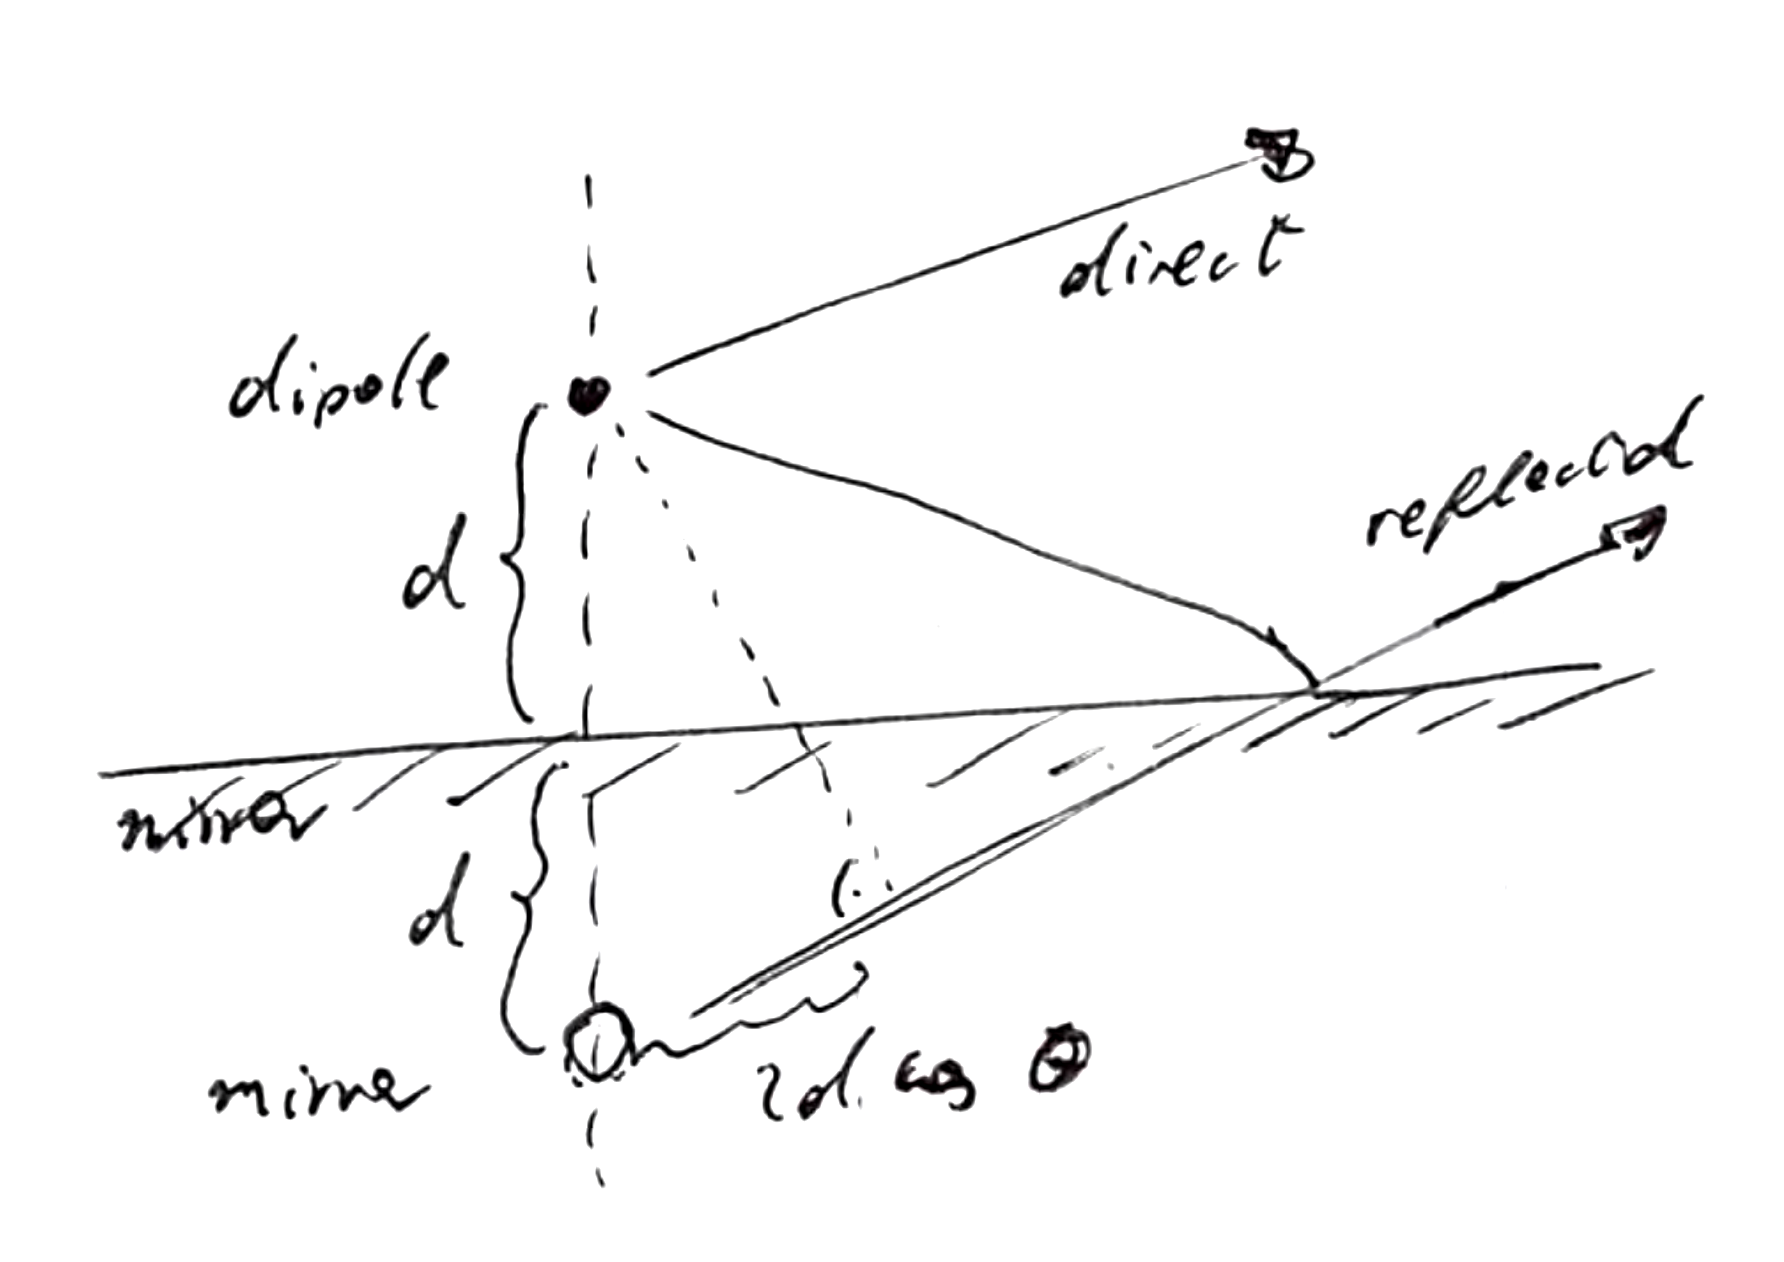
\includegraphics[width=\textwidth]{\currfiledir/drexhage-sketch.png}
\caption{Two paths of emission interfere at the observer. This can be seen as additional emission of an image dipole.}
\end{marginfigure}

Following the notation of \cite{Langguth16}, the field at the observer in distance $R$ can be written as
\begin{equation}
E(R) \propto \frac{e^{i \, k \, R}}{R} \, S(\theta, \phi) \, \left( e^{i \phi} + r  e^{- i \phi} \right)
\end{equation}
where $r$ is the (Fresnel) reflection coefficient of the surface and $\pm \phi = \pm k d \cos \theta$ the phase difference between the two paths. $S(\theta, \phi)$ describes the dipolar emission pattern. Now we assume a perfect reflection ($r=1$), abbreviate  the phase difference by $x = 2 k d$ and integrate over the half space above the mirror. One gets
\begin{eqnarray}
 \frac{\gamma_\perp }{\gamma_0} & = & 1 + 3 \left( - \frac{\cos x}{x^2} + \frac{\sin x}{x^3} \right) \\
  \frac{\gamma_\parallel }{\gamma_0} & = & 1 + \frac{3}{2} \left( - \frac{\sin x}{x} - \frac{\cos x}{x^2}  + \frac{\sin x}{x^3} \right) 
\end{eqnarray}
For completeness, the relative shift of the eigen-frequencies in this case are
\begin{eqnarray}
 \frac{\Delta \omega_\perp }{\gamma_0} & = & - \frac{3}{2} \left(  \frac{\sin x}{x^2} + \frac{\cos x}{x^3} \right) \\
  \frac{\Delta \omega_\parallel }{\gamma_0} & = & \frac{3}{4} \left(  \frac{\cos x}{x} - \frac{\sin x}{x^2}  - \frac{\cos x}{x^3} \right) 
\end{eqnarray}





\printbibliography[segment=\therefsegment,heading=subbibliography]
